\chapter[Diseño y desarrollo de la aplicación]{Diseño y desarrollo de la aplicación para adaptación de recetas}
\label{ch:Consultas_Adaptadas}

\begin{quote}
  Este capítulo recoge el comportamiento del módulo de Consultas adaptadas, así como la descripción del prototipo de aplicación que se ha implementado para ilustrar el funcionamiento del sistema de adaptación de dietas con la herramienta de fusión de datos heterogéneos.
\end{quote}


\section{Recomendación de recetas}

La recomendación de las recetas es un campo concreto de estudio dentro de los sistemas de recomendación en Food Computing, el cual se centra fundamentalmente en la recomendación de dietas cuyas recetas cumplen una serie de características nutricionales. Entre otras muchas especificaciones, destacan las dietas saludables o aquellas que persiguen un objetivo concreto, como puede ser la pérdida de peso o la definición de masa muscular.

Dentro del amplio campo de estudio de recomendación de recetas, destacan dos formas principales: la recomendación de recetas ya existentes, y la recomendación de recetas a partir de generación automática de recetas~\cite{chen2019eating}. En el primer caso hablamos de recomendación de recetas ya existentes donde los sistemas, en base a unas preferencias concretas, realizan un filtrado hasta proporcionar la receta o conjunto de ellas que mejor se adapten a los requerimientos del usuario. Se han desarrollado una gran cantidad de sistemas de recomendación basados en recetas desde el punto de vista de Recomendación basada en el contenido, en función de  la puntuación y opinión que los usuarios tienen de los ingredientes que las forman~\cite{Freyne:2010:IFP:1719970.1720021,a3e625bf40904a799c3b8e35929388b7}.
En cuanto a los sistemas de recomendación dependiente del contexto, se han desarrollado sistemas que aconsejan recetas en base al género, tiempo, aficiones, localización u otros aspectos culturales relacionados con los usuarios. También hay distintos sistemas de recomendación que tienen en cuenta distintas combinaciones de sabores, o incluso patrones de combinación de ingredientes en las distintas recetas, y otros basados en otro tipo de datos que en principio puedan parecer menos relevantes, como la rutina diaria de usuarios obtenida a partir de redes sociales como Twitter~\cite{Rokicki2016PlateAP}. En el segundo caso hablamos de sistemas generadores de recetas automáticas: a partir del estudio de las relaciones que existen entre ingredientes, recetas y factores multiculturales en las cocinas, se pueden generar versiones de recetas que permitan mantener dicha coherencia intrínseca contenida en las recetas~\cite{10.3389/fict.2018.00014}. En este capítulo, nos centramos en este segundo caso.


Además, es relevante destacar que la incorporación de aspectos saludables en los sistemas de recomendación de dietas tiene especial importancia, y, debido a la gran cantidad de literatura centrada en la incorporación de este factor a los sistemas de recomendación, merece ser destacada en este apartado. En los últimos años, se ha producido un auge en el desarrollo de sistemas de recomendación centrados en la generación automática de dietas personalizadas teniendo como requisito que sean saludables~\cite{burilo2019nutricion,Trattner2017}. 



\subsubsection{Aplicaciones móviles de recomendación de recetas}

Utilizar aplicaciones móviles para resolver problemas de Food Computing ha resultado exitoso, mostrando su efectividad en ensayos focalizados a la adecuación del consumidor hacia dietas más saludables~\cite{ipjian2017smartphone}. Los sistemas de Food Computing cada vez se encuentran más inmersos en las aplicaciones móviles, dando lugar a múltiples aplicaciones con funcionalidades muy diversas. El desarrollo de las comunidades de usuarios online en las que se comparten millones de recetas (AllRecipes y Yummly) ha contribuido a la disponibilidad de su información a través de aplicaciones móviles más allá de mantener su servicio vía web. Sin embargo, estos servicios están muy focalizados a la búsqueda de recetas, y no a su recomendación y adaptación a los usuarios, lo cual es una de las funcionalidades más demandadas desde estas aplicaciones~\cite{chen2019eating}. En esta línea, han surgido sistemas centrados en la recomendación de recetas a través de dispositivos móviles~\cite{cheng2014content,johnson2014mobile,ketmaneechairat2017recommender,maruyama2012real}. 

La falta de información (normalmente nutricional) muy concreta o específica que se suele proporcionar en las recetas procedentes de esas fuentes de datos ha originado que éstas no tenga cabida en que los sistemas de recomendación de recetas ya existentes, ya que las características de estos conjuntos de datos no son lo suficientemente detalladas como para poder trabajar con restricciones muy específicas que no se proporcionen en ámbitos poco especializados. Es por ello que la generación y completación de recetas ha sido y es la vía de recomendación de recetas más utilizada en este ámbito, utilizando para ello las relaciones existentes entre ingredientes y recetas~\cite{de2016data}. En este contexto podemos destacar el framework \textit{NutRec}, cuyo motor principal en un sistema de recomendación basado en la búsqueda de recetas similares a una pseudo-receta generada automáticamente a partir de las especificaciones concretas del usuario.

\section{Adaptación de recetas según restricciones}

Como ya se ha ido introduciendo a lo largo del desarrollo de este proyecto, para ilustrar el funcionamiento del sistema desarrollado se ha implementado un módulo de Consultas Adaptadas, el cual, en nuestro caso, permite adecuar recetas en función de unas restricciones alimenticias dadas. Para ello, se permite seleccionar una receta y una restricción con el objetivo de detectar sus ingredientes y modificarlos en caso de que la información nutricional de alguno (o varios) de ellos impida su uso en en algún tipo de dieta (como puede ser la vegetariana). 

En este último módulo del sistema se hace uso de fuentes de datos heterogéneas que se fusionan mediante los dos módulos anteriores explicados en el Capítulo \ref{ch:Capitulo 5} y \ref{ch:Capitulo 6}. De esta forma, con una única consulta podremos obtener todos los datos necesarios para que este módulo pueda funcionar correctamente. En la Figura \ref{fig:datos-agregados} se visualiza esta misma idea.

\begin{figure}[H]
    \centering
    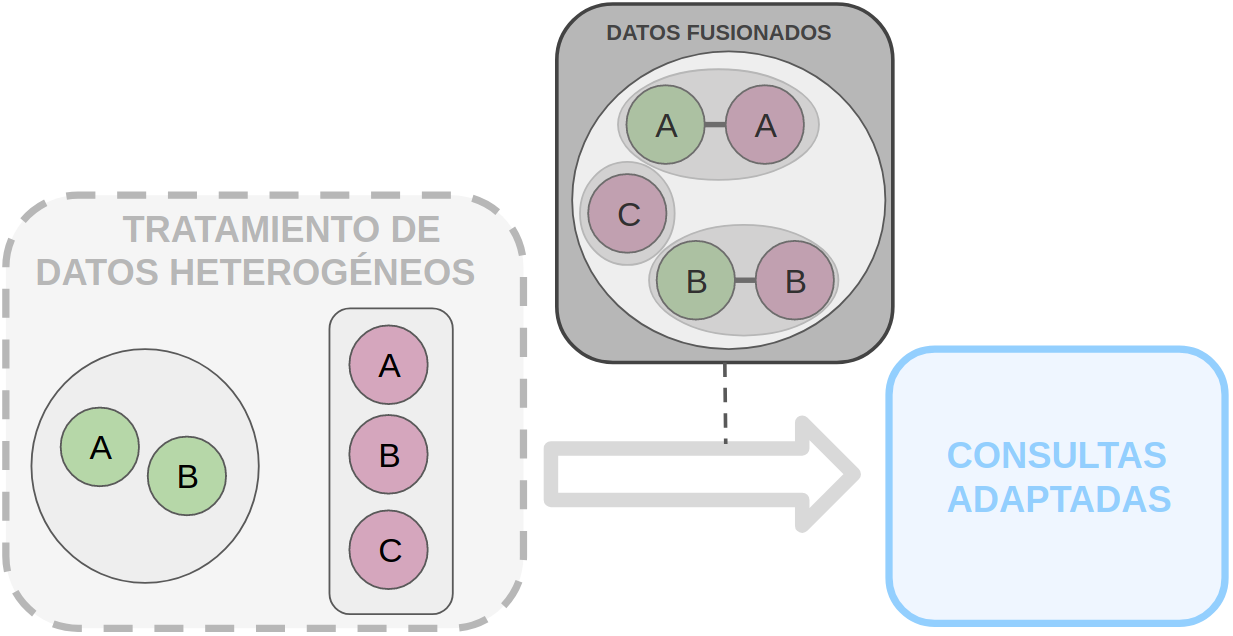
\includegraphics[width=1.0\textwidth]{imagenes/arquitectura/datos-agregados.png}
    \caption{Consulta sobre los datos fusionados}
    \label{fig:datos-agregados}
\end{figure}


Centrándonos en nuestro problema de adaptación de dietas, se utilizan dos fuentes de datos: una primera formada por recetas, y una segunda base de datos con información nutricional, ambas detalladas en el apartado \ref{sec:bd_recetas}. Al conectar las recetas con la base de datos nutricional (a través de sus ingredientes), podremos extrapolar dicha información y obtener las características nutricionales de las recetas (ver Figura \ref{fig:mapping-entre-recetas-1}). De esta forma, se podrá comprobar si los ingredientes cumplen o no las restricciones impuestas (y en su caso, modificarlos por otros más adecuados). Es en este punto es donde toma relevancia el tratamiento de datos heterogéneos, que nos permite obtener información especializada que no viene incluida en los datos de las recetas. 


\begin{figure}[H]
    \centering
    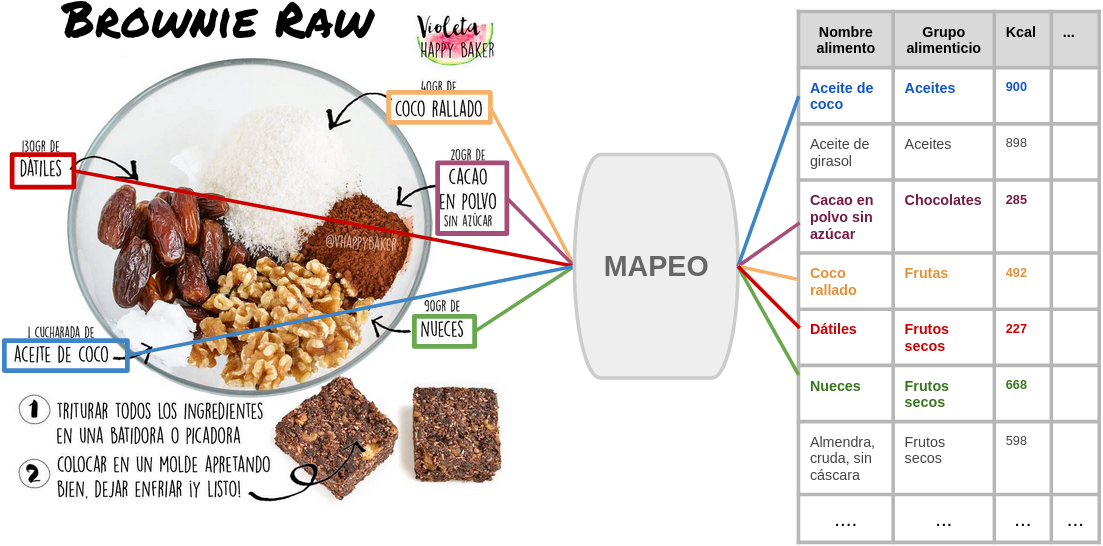
\includegraphics[width=1.0\textwidth]{imagenes/app/MAPEO ENTRE DATOS.png}
    \caption{Mapeo de datos de fuentes heterogéneas}
    \label{fig:mapping-entre-recetas-1}
\end{figure}


\section{Aplicación móvil}
Para ilustrar cómo funciona la solución diseñada para el problema de adaptación de recetas, se ha diseñado un prototipo funcional de aplicación móvil que permita ver su comportamiento de una forma más cómoda y realista, coherente a la línea que se sigue hoy en día con este tipo de pseudo-recomendaciones.


\subsection{Arquitectura}

En la Figura \ref{fig:arquitectura-app} se muestra la arquitectura global de la aplicación de adaptación de recetas. A través de la interfaz móvil, se realizan consultas al sistema de adaptación de recetas realizando consultas a la API, para obtener recetas adecuadas a las restricciones. A su vez, se hace uso de una base de datos de recetas, también accesible desde la API.

\begin{figure}[H]
    \centering
    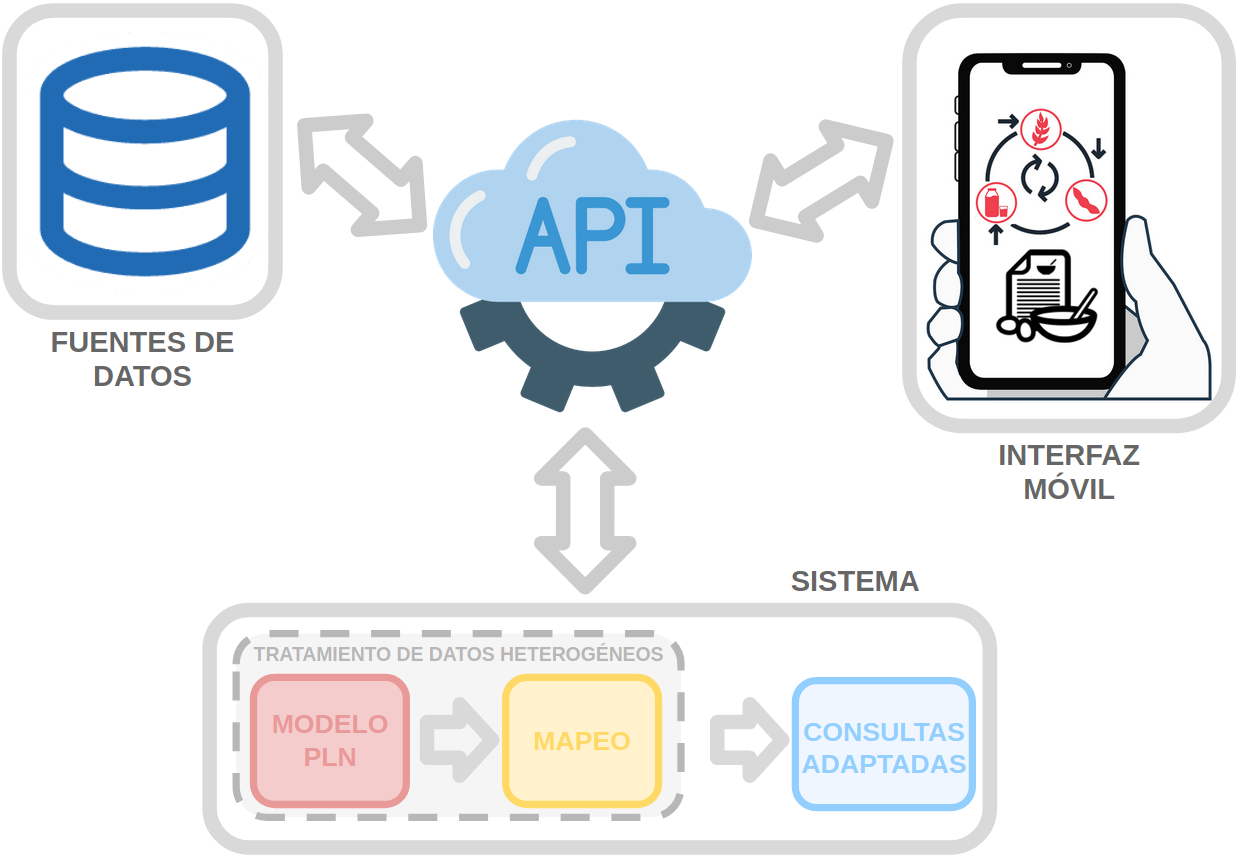
\includegraphics[width=1.0\textwidth]{imagenes/app/arq.png}
    \caption{Arquitectura de la aplicación}
    \label{fig:arquitectura-app}
\end{figure}

\subsection{Tecnologías utilizadas}

A continuación se enumeran las tecnologías utilizadas para la implementación y puesta en funcionamiento del sistema descrito.

\begin{enumerate}
    \item Para la Interfaz de Programación de Aplicaciones (API) se ha utilizado el lenguaje de programación Python con la librería Flask (\url{https://flask.palletsprojects.com/en/1.1.x/}).
    
    \item Para la base de datos se ha utilizado MongoDB (\url{www.mongodb.com/es}), un sistema de base de datos no estructuradas, orientado a colecciones de documentos. 
    
    \item Para la implementación de la aplicación, se ha utilizado IONIC  (\url{https://ionicframework.com/}), un kit de desarrollo Software de código abierto, el cual permite la creación de aplicaciones a nivel web y móvil (tanto para el sistema operativo Android como iOS). 
    
\end{enumerate}


\subsection{Fuentes de datos}\label{sec:bd_recetas}
Para el funcionamiento correcto del módulo, es necesario utilizar una base de datos que permita gestionar las recetas así como una base de datos de composición alimenticia para obtener la información nutricional de los alimentos.

\subsubsection{Base de datos de recetas}
En nuestro caso, hemos utilizado recetas procedentes de una colección de Food.com\footnote{\url{www.food.com}} proporcionada por Kaggle. Esta colección se llama  \textit{Food.com Recipes and Interactions}, que tal y como indica su nombre, está orientada al estudio de recetas e interacciones entre usuarios\footnote{\url{www.kaggle.com/shuyangli94/food-com-recipes-and-user-interactions}}. Puesto que no necesitamos las interacciones de los usuarios, únicamente hemos importado el fichero correspondiente a las recetas sin preprocesar (RAW\_recipes.csv\footnote{\url{www.kaggle.com/shuyangli94/food-com-recipes-and-user-interactions\#RAW\_recipes.csv}}).

La elección de este conjunto de datos viene dada por el origen de las recetas que lo forman. Esta colección no contiene ninguna receta procedente de las páginas web de las que se obtiene el conjunto de recetas del corpus con el que se entrena el modelo de Word Embedding. De esta forma, aseguramos que nuestros resultados con este módulo son válidos y no están sesgados por las recetas que utilizamos, pues no se han empleado para la construcción del modelo del lenguaje. Además, el contenido de dichas recetas está en inglés (recordemos que el modelo de lenguaje implementado está en dicho idioma) e incluyen todos los atributos de recetas requeridos por el módulo.

Para gestionar la base de datos de recetas, hemos utilizado tres colecciones de datos:
\begin{itemize}
    \item \textbf{Colección de recetas originales}: esta colección almacena todas las recetas utilizadas para el sistema de adaptación de recetas. Antes de insertar las recetas en la base de datos, hemos prescindido de aquellas columnas del conjunto de Kaggle que no nos aportan información útil, quedándonos únicamente con aquellas que sí nos interesa utilizar en el Módulo de Consultas Adaptadas. Asimismo, hemos añadido un campo \textit{Imagen}, para mejorar la visualización en el prototipo. En la Tabla \ref{table:ejemplo_receta} se muestra el contenido de las recetas de esta colección.
    
    \item \textbf{Colección de recetas adaptadas}: esta colección almacena recetas ya adaptadas a una restricción mediante el Módulo de Consultas Adaptadas. Contiene la misma estructura de atributos detallada en la sección anterior (ver Tabla \ref{table:ejemplo_receta}), con dos diferencias: en primer lugar, añade un atributo para almacenar la restricción aplicada sobre la receta y, en segundo lugar, los atributos \textit{Ingredientes} y \textit{Pasos en la aplicación} contienen dos nuevos campos, que almacenan si existe una modificación y, en caso afirmativo, de cuál se trata.
    
    \item \textbf{Colección de etiquetas de recetas}: una de las ventajas del conjunto de datos utilizado es que las recetas contienen un campo \textit{Etiquetas} que permite realizar clasificaciones sobre ellas. En nuestro caso, hemos definido una colección de etiquetas con algunas de las utilizadas en las recetas con el fin de poder clasificarlas en base a las etiquetas que nos sean de utilidad y realizar consultas por medio de ellas. Esta colección contiene la etiqueta, con un nombre e imagen añadida por nosotros para mejorar la de visualización en el prototipo.
    
\end{itemize}

\setlength{\tabcolsep}{2pt} 
\begin{table}[H]
\begin{tabular}{p{0.17\textwidth}|p{0.5\textwidth}|p{0.27\textwidth}}
\textbf{Atributo} & \textbf{Contenido} & \textbf{Tipo} \\ \hline 
Descripción & Descripción de la receta, consejos y algunos comentarios extra & cadena de caracteres \\
% Identificador de receta & Identificador de la receta en la colección & cadena de caracteres \\
Imagen & Imagen de la receta & cadena de caracteres \\
Nombre & Nombre de la receta & cadena de caracteres \\
Ingredientes & Lista de ingredientes de la receta & lista de cadena de caracteres \\
Minutos & Tiempo de preparación de la receta en minutos & cadena de caracteres \\
% n\_ingredients & Número de ingredientes en la receta & número entero \\
% n\_steps & Número de pasos en la preparación de la receta & número entero \\
Nutrientes & Lista con los valores nutricionales de la receta en el siguiente orden: kilocalorías, grasas totales, azúcar, sodio, proteína, grasas saturadas y carbohidratos & lista de números de coma flotante \\
Pasos en la preparación & Lista con los pasos para preparar la receta & lista de cadenas de caracteres \\
Etiquetas & Lista de etiquetas asociada a la receta (p.ej., ``30 minutes or less'') & lista de cadenas de caracteres
\end{tabular}
\caption{\label{table:ejemplo_receta} Descripción de los campos en la colección de recetas originales}
\end{table}


\subsubsection{Base de datos de Composición de Alimentos}

Como se ha comentado previamente, este módulo requiere un procedimiento previo de tratamiento de datos heterogéneos de las recetas con una base de datos de composición de alimentos para obtener información nutricional de los ingredientes que forman las recetas. En este módulo se ha utilizado la Base de Datos de Composición de Alimentos i-Diet~\cite{iDietrf}, que se encuentra detallada en el Capítulo \ref{ch:Pruebas} (Apartado \ref{subsec:idiet}). 

La elección de i-Diet se debe principalmente a dos de sus características principales. Por un lado se trata de una base de datos de alimentos muy depurada que además de ser utilizada por nutricionistas, se emplea en sistemas informáticos de nutrición y dietética~\cite{iDietrf}. Por otro lado, está orientada a su uso conjunto con platos (lo cual es difícil de encontrar en este ámbito), por lo que contiene una cantidad representativa de ingredientes que suelen aparecer en recetas de cocina.


\subsection{Sistema para Adaptación de Recetas}

Para poder llevar a cabo la adaptación de las recetas en base a una restricción alimenticia dada se siguen los siguientes pasos:
\begin{enumerate}
    \item En primer lugar, se debe seleccionar una receta junto con la restricción alimenticia a aplicar, los cuales son los datos de entrada al sistema. En nuestro caso, esta receta se selecciona de entre una lista proporcionada. De esta receta, obtenemos sus ingredientes, de los cuales obtenemos sus correspondientes representaciones vectoriales con el Módulo de Procesamiento de Lenguaje Natural. 
    
    \item Una vez tenemos las representaciones vectoriales de los ingredientes se realiza un mapeo de estos alimentos hacia la base de datos de composición nutricional, para obtener información específica de cada uno de dichos alimentos. Este paso se lleva a cabo en el Módulo de Mapeo.
    
    \item Con toda la información de los ingredientes ya disponible, realizamos una consulta para ver cuales de ellos cumplen con las restricciones alimenticias proporcionadas (actualmente, el sistema incorpora dos restricciones a elegir: dieta vegana y dieta vegetariana). Para cada alimento que no la cumpla, se vuelve a recurrir al módulo de mapeo, para recomendar un posible alimento que pueda sustituirlo. En este paso, al usar las representaciones capaces de capturar la información semántica de los ingredientes, se posibilita que la opción proporcionada se adapte a dicha receta, puesto que este segundo mapeo se realiza únicamente sobre los elementos permitidos devolviendo el más cercano al ingrediente a modificar. Finalmente, se proporciona como la salida, la receta con los cambios correspondientes. En nuestro caso, en vez de proporcionar una única alternativa, hemos decidido facilitar varias opciones de reemplazo para cada ingrediente incompatible. Con ello, se da la posibilidad de elegir entre uno de ellos o realizar alguna modificación previa a la adaptación final de la receta. 
\end{enumerate}


\subsection{Interfaz de Programación de Aplicaciones (API)}

La Interfaz de Programación de Aplicaciones permite acceder a través de peticiones a las operaciones CRUD sobre las recetas, además de conectarse al sistema de adaptación de recetas y poder realizar las adaptaciones que se requieran (ver Figura \ref{fig:arquitectura-app}). 

\subsubsection{Operaciones CRUD}

Se ha realizado el diseño e implementación de una API REST completamente funcional, que se conecta a las colecciones de la base de datos para realizar operaciones sobre los datos almacenados. Para ello, se han definido rutas con todas las consultas necesarias para el funcionamiento de la aplicación tanto a nivel de receta como de colección: lista completa de recetas, recetas que incluyan alguna etiqueta concreta, etc. Para poder realizar peticiones a nivel de receta, se ha llevado a cabo el diseño del correspondiente modelo de datos de Receta, para describir el objeto Receta y poder trabajar con la estructura de los datos en las colecciones de recetas. Este objeto Receta se utiliza para llevar a cabo las operaciones CRUD correspondientes para crear, leer, actualizar y eliminar recetas de la base de datos.


\subsubsection{Adaptación de recetas}

Se han implementado las rutas necesarias para poder realizar peticiones al Sistema de Adaptación de recetas, y así obtener recetas adaptadas acorde a alguna restricción concreta. Para ello, a través de la API se cargan los modelos predictivos necesarios para poder llevar a cabo dichas acciones.

\subsection{Aplicación}

\subsubsection{Diseño conceptual}

Previa a la implementación del prototipo que se utiliza en esta aplicación, se ha llevado a cabo el diseño conceptual de la aplicación. En primer lugar, las capacidades de la aplicación se pueden ver en el diagrama de casos que se ha obtenido para esta aplicación (ver Figura \ref{fig:diagrama_casos}). Si nos centramos en la arquitectura de la información, se han descrito las tareas usando un diagrama de tareas HTA (ver Figura \ref{fig:diagramahta}). Los posibles planes para el diagrama HTA se enumeran a continuación:
\begin{enumerate}
    \item \textbf{Plan 0}: Si sólo quiere consultar recetas
    \begin{enumerate}
        \item Hacer 1-2-3-4-5-6-8 (7 opcional)
    \end{enumerate}
    \item \textbf{Plan 1}: Si quiere adaptar recetas
        \begin{enumerate}
        \item Hacer 1-2-3-4-5-6-8 (7 opcional)
        \item Si quiere guardar la receta hacer 6.3
    \end{enumerate}
\end{enumerate}


El contenido de la información se ha descrito mediante un diagrama de conceptos (ver Figura \ref{fig:diagrama_conceptual}), en el que se puede apreciar las relaciones existentes entre las recetas (originales y adaptadas) y el usuario en cuestión. Por último, se han descrito los mapas de flujo para el usuario de la aplicación móvil a través de un diagrama WireFlow que se puede ver en la Figura \ref{fig:diagrama_wireflow}.

En base a estos diagramas, se puede apreciar que la funcionalidad implementada en la aplicación se corresponde con una tarea: la adaptación de recetas. Por ello, queremos resaltar que estos diagramas (y por tanto, la aplicación) podrían integrarse en el diseño de una aplicación móvil de dietética más general, en la que entre otras muchas tareas, una de las facilitadas fuera la adaptación en base a restricciones del usuario.


\begin{figure}[H]
    \centering
    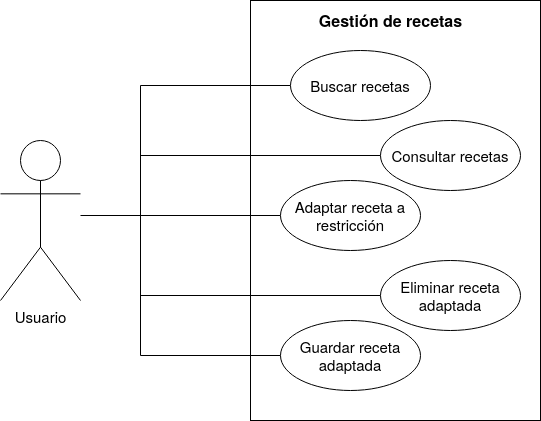
\includegraphics[width=0.6\textwidth]{imagenes/app/diagramas/Casos de uso.png}
    \caption{Diagrama de casos de uso de la aplicación}
    \label{fig:diagrama_casos}
\end{figure}


\begin{figure}[H]
    \centering
    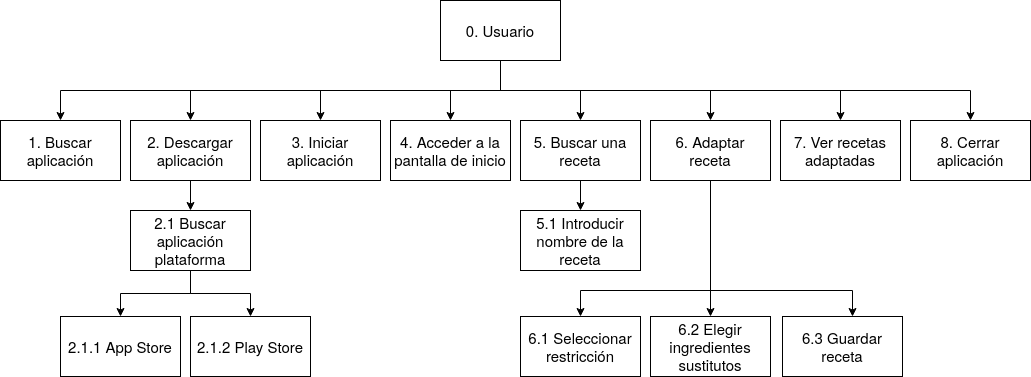
\includegraphics[width=1.0\textwidth]{imagenes/app/diagramas/diagrama-hta.png}
    \caption{Diagrama HTA de la aplicación}
    \label{fig:diagramahta}
\end{figure}



\begin{figure}[H]
    \centering
    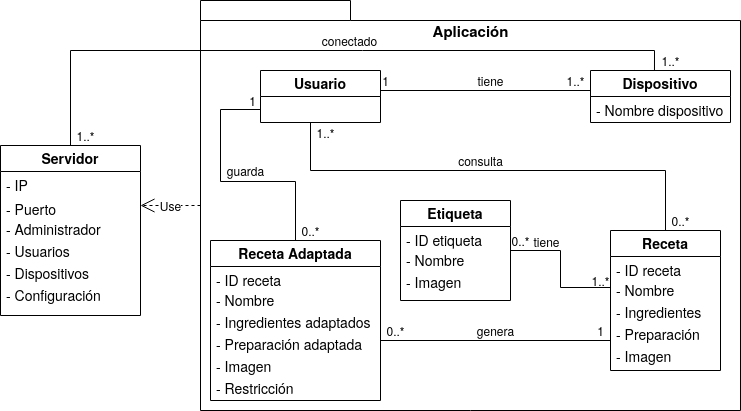
\includegraphics[width=1.0\textwidth]{imagenes/app/diagramas/diagrama_conceptual.png}
    \caption{Diagrama Conceptual de la aplicación}
    \label{fig:diagrama_conceptual}
\end{figure}


\begin{figure}[H]
    \centering
    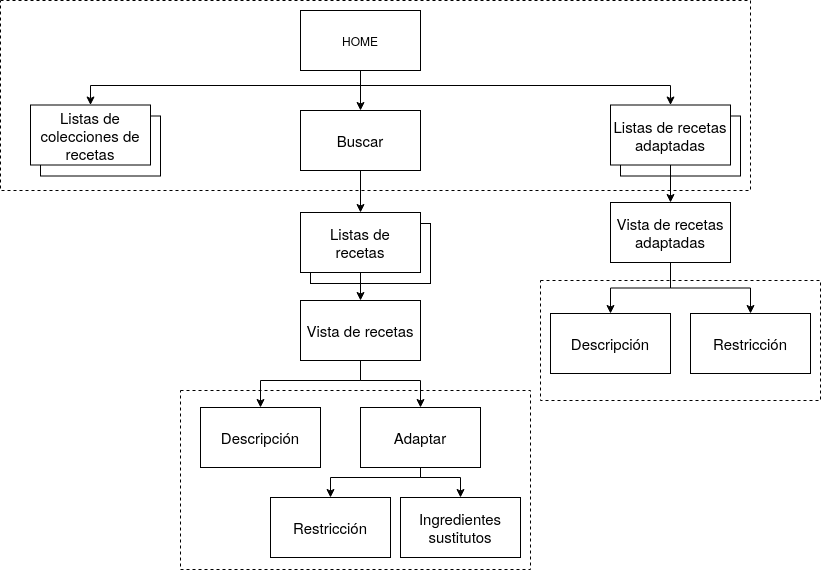
\includegraphics[width=1.0\textwidth]{imagenes/app/diagramas/Wireflow.png}
    \caption{Diagrama Wireflow de la aplicación}
    \label{fig:diagrama_wireflow}
\end{figure}

\subsubsection{Funcionamiento de la aplicación}
En la selección de Figuras \ref{fig:ejemplo_uso} se puede ver el comportamiento básico de la aplicación, el cual consiste en acceder a una receta y obtener su versión adaptada. Tal y como se puede ver, a partir de la navegación por colecciones de recetas (Figura \ref{fig:pantallas_basicas_1}), se puede acceder a una receta específica (Figura \ref{fig:pantallas_basicas_2}) y obtener una adaptación de la misma (Figura \ref{fig:pantallas_basicas_3}). Estas tres pantallas de la aplicación tan sólo forman una versión simplificada del funcionamiento de la aplicación. En el Apéndice \ref{ch:Anexo_Pantallas} se puede ver de forma detallada toda la estructura de navegación en esta aplicación a través de los flujos de datos entre las distintas pantallas implementadas. 

\begin{figure}[H]
    \centering
    
    \begin{subfigure}[b]{0.322\linewidth}
        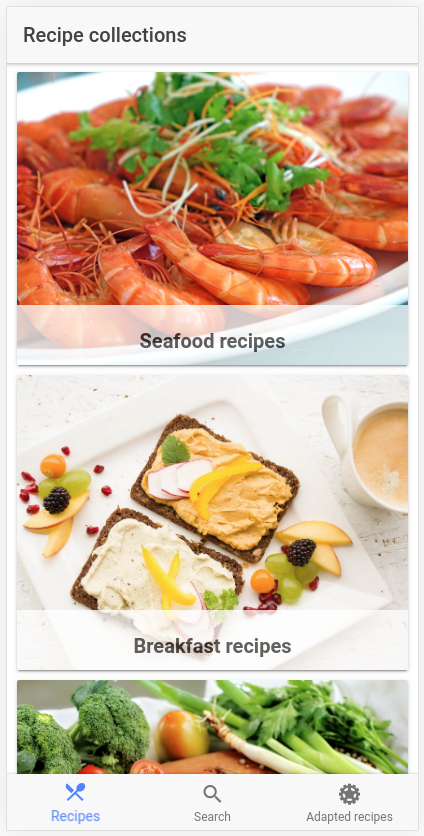
\includegraphics[width=\linewidth]{imagenes/app/pantallas/app_1.png}
        \caption{Colecciones}
        \label{fig:pantallas_basicas_1}
    \end{subfigure}
    \begin{subfigure}[b]{0.32\linewidth}
        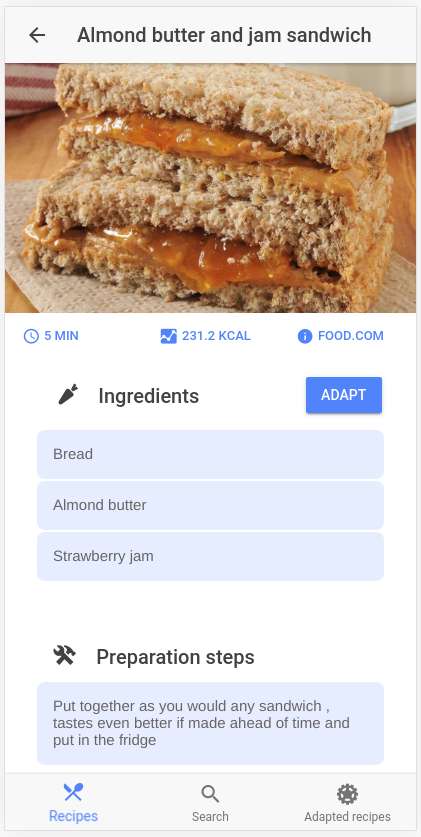
\includegraphics[width=\linewidth]{imagenes/app/pantallas/app_2.png}
        \caption{Receta original}
        \label{fig:pantallas_basicas_2}
    \end{subfigure}
    \begin{subfigure}[b]{0.32\linewidth}
        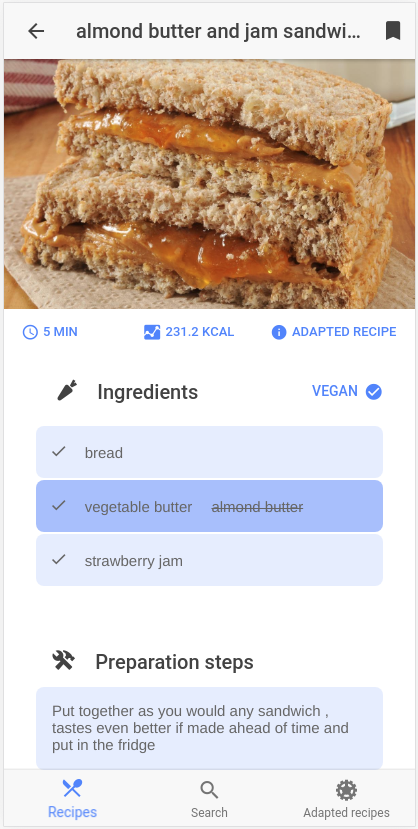
\includegraphics[width=\linewidth]{imagenes/app/pantallas/app_3.png}
        \caption{Receta adaptada}
        \label{fig:pantallas_basicas_3}
    \end{subfigure}
    \caption{Pantallas de la aplicación: funcionamiento básico}
    \label{fig:ejemplo_uso}
\end{figure} 

\subsection{Siguientes pasos en el desarrollo de la aplicación móvil}

Tal y como se ha visto en la sección anterior, a pesar de que la funcionalidad básica está implementada, aún queda un amplio recorrido para obtener una versión final de la interfaz gráfica de esta aplicación móvil, ya que, tal y como se ha descrito, se encuentra en una primera iteración del proceso de desarrollo. Con este prototipo pretendemos centrarnos en la funcionalidad, no sólo con el objetivo de ver el funcionamiento de la inteligencia por debajo de la aplicación, sino también para ver las posibilidades que tienen los sistemas adaptados tal como el que se ha implementado en este trabajo. 

Para continuar con el diseño de la interfaz, los pasos a seguir parten de la evaluación de la aplicación con y sin usuarios: en primer lugar una evaluación general, con lista de chequeos y los consecuentes informes de evaluación heurística, seguidos del test de usabilidad de la aplicación y finalmente, un test de evaluación con usuarios para analizar el éxito y dificultades al interactuar con la aplicación. A través de estas evaluaciones, se podrán realizar las siguientes iteraciones, más centradas en el diseño y ultimación de las funcionalidades de la aplicación con lo que esperan los usuarios finales.

